\section{Research Questions and Hypotheses}

There is a general lack of research into the problem of VR head collisions. Current VR developers experiment with various solutions in their games, and all of these methods have their advantages and disadvantages. There is a disagreement in VR developers community over which solution should be used in future games. Some developers wonder if it is even worth the effort to implement any solution at all. Therefore, the goal of this study is to examine different solutions and to determine which one of them is best suited for modern VR games.
 
There are several possible solutions to the problem of VR head collisions, and they can be implemented in many different ways. Due to time constraints, only the following four most popular methods were chosen for this study:

\begin{itemize}
\item Screen fade: When the head collision is detected, the whole screen fades to black in the span of a second. The view remains blacked-out for as long as the player's head collides with the object.
\item Delayed push-back: If the player keeps colliding with the object for longer than a second, he is slowly pushed backwards until he leaves the object's boundaries.
\item Instant push-back: When the user starts to collide with some obstacle, a collision vector is computed and its projection on the horizontal plane is immediately added to the player's position. This effectively moves the user away from the object, preventing him from ever looking inside it.
\item Teleportation: If the collision is detected and maintained for the duration of a second, the player is instantly teleported to the last know valid position. 
\end{itemize}

The quality of VR experience is affected by many factors. VR sickness, the sense of presence in virtual world, and the usability of the user interface are some of the main considerations in designing comfortable VR experience. Some developers consider different factors to be more important than others. For this reason, the proposed solutions to the problem of VR head collisions are examined from three different perspectives. The answers to the following research questions will help VR developers decide which particular solution to use:

\begin{itemize}
\item RQ1: How the proposed solutions to the problem of VR head collisions affect the virtual reality sickness?
\item RQ2: How the proposed solutions to the problem of VR head collisions affect the sense of presence?
\item RQ3: How usable are the proposed solutions to the problem of VR head collisions?
\end{itemize}

Three null hypotheses corresponding to the research questions are as follows:

\begin{itemize}
\item H$_{\text{01}}$: All proposed solutions to the problem of VR head collisions have the same effect on the virtual reality sickness.
\item H$_{\text{02}}$: All proposed solutions to the problem of VR head collisions have the same effect on the sense of presence.
\item H$_{\text{03}}$: All proposed solutions to the problem of VR head collisions have the same level of usability.
\end{itemize}

The null hypotheses are tested against the following three alternative hypotheses:

\begin{itemize}
\item H$_{\text{A1}}$: Some proposed solutions to the problem of VR head collisions have more positive effect than others on the virtual reality sickness.
\item H$_{\text{A2}}$: Some solutions to the problem of VR head collisions have more positive effect than others on the sense of presence.
\item H$_{\text{A3}}$: Some solutions to the problem of VR head collisions have higher level of usability than others.
\end{itemize}

\section{Questionnaires}

Two questionnaires were prepared for the study. Before the experiment began, participants were asked to fill in a demographic questionnaire. It included information about age, gender, previous experience with VR, and previous experience with motion sickness (see Appendix A). Each time after testing one of the solutions to the problem of VR head collisions, the participants filled in a post-test questionnaire (see Appendix B). This questionnaire is composed of three sections, which correspond accordingly to the three research questions. First, the participants described what VR sickness symptoms they felt during the experiment (see question 2 in Appendix B). Next, they answered to six questions about the sense of presence in the virtual environment (see questions 3-8 in Appendix B). Finally, the participants rated the tested method with eight usability factors on the scale from 1 to 5 (see question 9 in Appendix B).

\subsection{Simulator Sickness Questionnaire}

The VR sickness section of post-test questionnaire was prepared using the Simulator Sickness Questionnaire (SSQ) \cite{SSQ}, a widely acknowledged standard for studying simulator sickness. The SSQ was developed in 1993 with the purpose of enhancing training efficiency in flight simulators. Due to the similarity of simulator sickness with VR sickness, in the recent years the SSQ was also used by many researchers studying comfortable VR locomotion \cite{TELEPORTATIONEFFECTS}\cite{NODEBASEDTELEPORTATION}\cite{SUSMETHODARTICLE}. The SSQ consists of 16 most commonly occurring simulator sickness symptoms: general discomfort, fatigue, headache, eye strain, difficulty focusing, salivation increasing, sweating, nausea, difficulty concentrating, "fullness of the head", blurred vision, dizziness with eyes open, dizziness with eyes closed, vertigo, stomach awareness, and burping. These symptoms fall into three different categories: nausea-related, oculomotor-related, and disorientation-related. Each questionnaire item is scored on a four point scale (0-3): none, slight, moderate, and severe. The scores for each category and the total SSQ score are multiplied by the following weight factors: nausea is multiplied by 9.54, oculomotor by 7.58, disorientation by 13.92, and total SSQ by 3.74.

\subsection{Presence Questionnaire}

The Slayer-Usoh-Steed (SUS) \cite{SUS} presence questionnaire was used to prepare the second section of post-test questionnaire. It was chosen for this study because it is the second most cited presence questionnaire applicable for VR \cite{SUSEVIDENCE}, and it has a relatively short list of six questions in comparison to other, longer questionnaires. All SUS questions are based on one of the three themes: the extent to which the virtual environment becomes the dominant reality, the sense of being in the virtual environment, and the extent to which the virtual environment is remembered as a ``place''. Each question is answered on a scale from 1 to 7, where the higher score indicates the greater sense of presence. The final presence score is a number of answers that have a score of 6 or 7.

\subsection{Usability Questionnaire}

In the usability section, the participants rated eight different factors: difficulty in understanding the method, difficulty in operating the method, feeling of being in control while using the method, required effort to use the method, feeling of tiredness while using the method, feeling of enjoyment while using the method, feeling of being overwhelmed while using the method, feeling of frustration while using the method. This exact approach was also used in two recent VR locomotion studies \cite{TELEPORTATIONSTUDY}\cite{NODEBASEDTELEPORTATION}. Each question was answered on a 5 point Likert scale, where 1 meant ``not at all'' and 5 meant ``very much''. The total usability score was calculated as follows: for each factor, except for the ``feeling of being in control'' and ``feeling of enjoyment'', the score was firstly subtracted from 5, and then it was added to the total score. In the two mentioned cases, the factor score was firstly subtracted by 1, and then it was added to the total score.

\section{Implementation}

The virtual environment used in the experiment was implemented using the Unity game engine (version 2018.3.6) \cite{UNITY}. Unity is a cross-platform engine that allows creating high-quality 3D games and natively supports VR development. The SteamVR Unity Plugin (version 1.2.3) \cite{STEAMVR}, a software development kit and application programming interface developed by Valve, was used to smoothly interface virtual reality headset with Unity. The plugin manages the following functions: loading 3D models for VR controllers, handling input from the controllers, and estimating what the hands look like while using those controllers. Additionally, the application used some functionality of the Virtual Reality Toolkit (VRTK) (version 3.3.0) \cite{VRTK}. VRTK is a collection of useful design patterns and pre-built assets that aid solving common problems found when building for virtual reality. It covers common solutions for locomotion within virtual space, interactions with virtual objects and UI elements, body physics, and much more. 

\subsection{Virtual Environment}

The virtual environment consisted of a large (30m x 30m), blue platform with 10 red objects: a box, a ladder, a pallet, a shed, a barrel, and five different trees (see Figure \ref{fig:veimplementation}). The platform was surrounded by short mountains to prevent users from wandering away from the designed experiment area. All 3D objects on the platform were imported from the free package found in the Unity Asset Store \cite{POLYGONCITY}. The platform itself was a scaled up cube model found in the default Unity assets. The terrain was generated by the Unity's built-in Terrain Engine.

\begin{figure}[th]
\centering
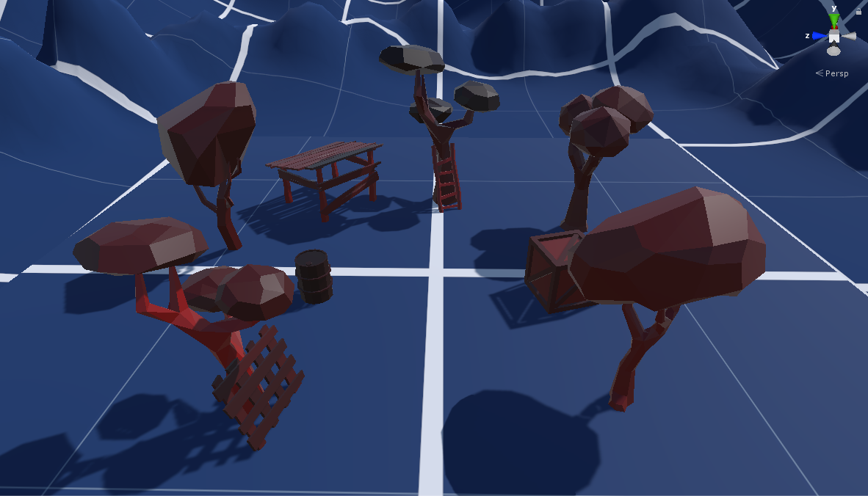
\includegraphics[width=1\textwidth]{img/virtual_environment.png}
\caption{The virtual environment used in the experiment: a large platform with 10 various objects on top.}
\label{fig:veimplementation}
\end{figure}

At the start of the application, the user of VR headset was placed in the center of the platform. The user could move through the virtual environment by using the ``Point \& Teleport'' locomotion technique. When the user pressed and held the trackpad on the controller, a blue teleportation curve appeared. He could then teleport by pointing with his hand and releasing the trackpad. The user could only teleport to areas on the platform that were not occupied by the 10 objects. When the area was not viable, the curve's color was changed from blue to red (see Figure \ref{fig:tpimplementation}). The teleportation locomotion was implemented with the help of VRTK\_HeightAdjustTeleport script \cite{VRTK_TELEPORT}.

\begin{figure}[th]
\centering
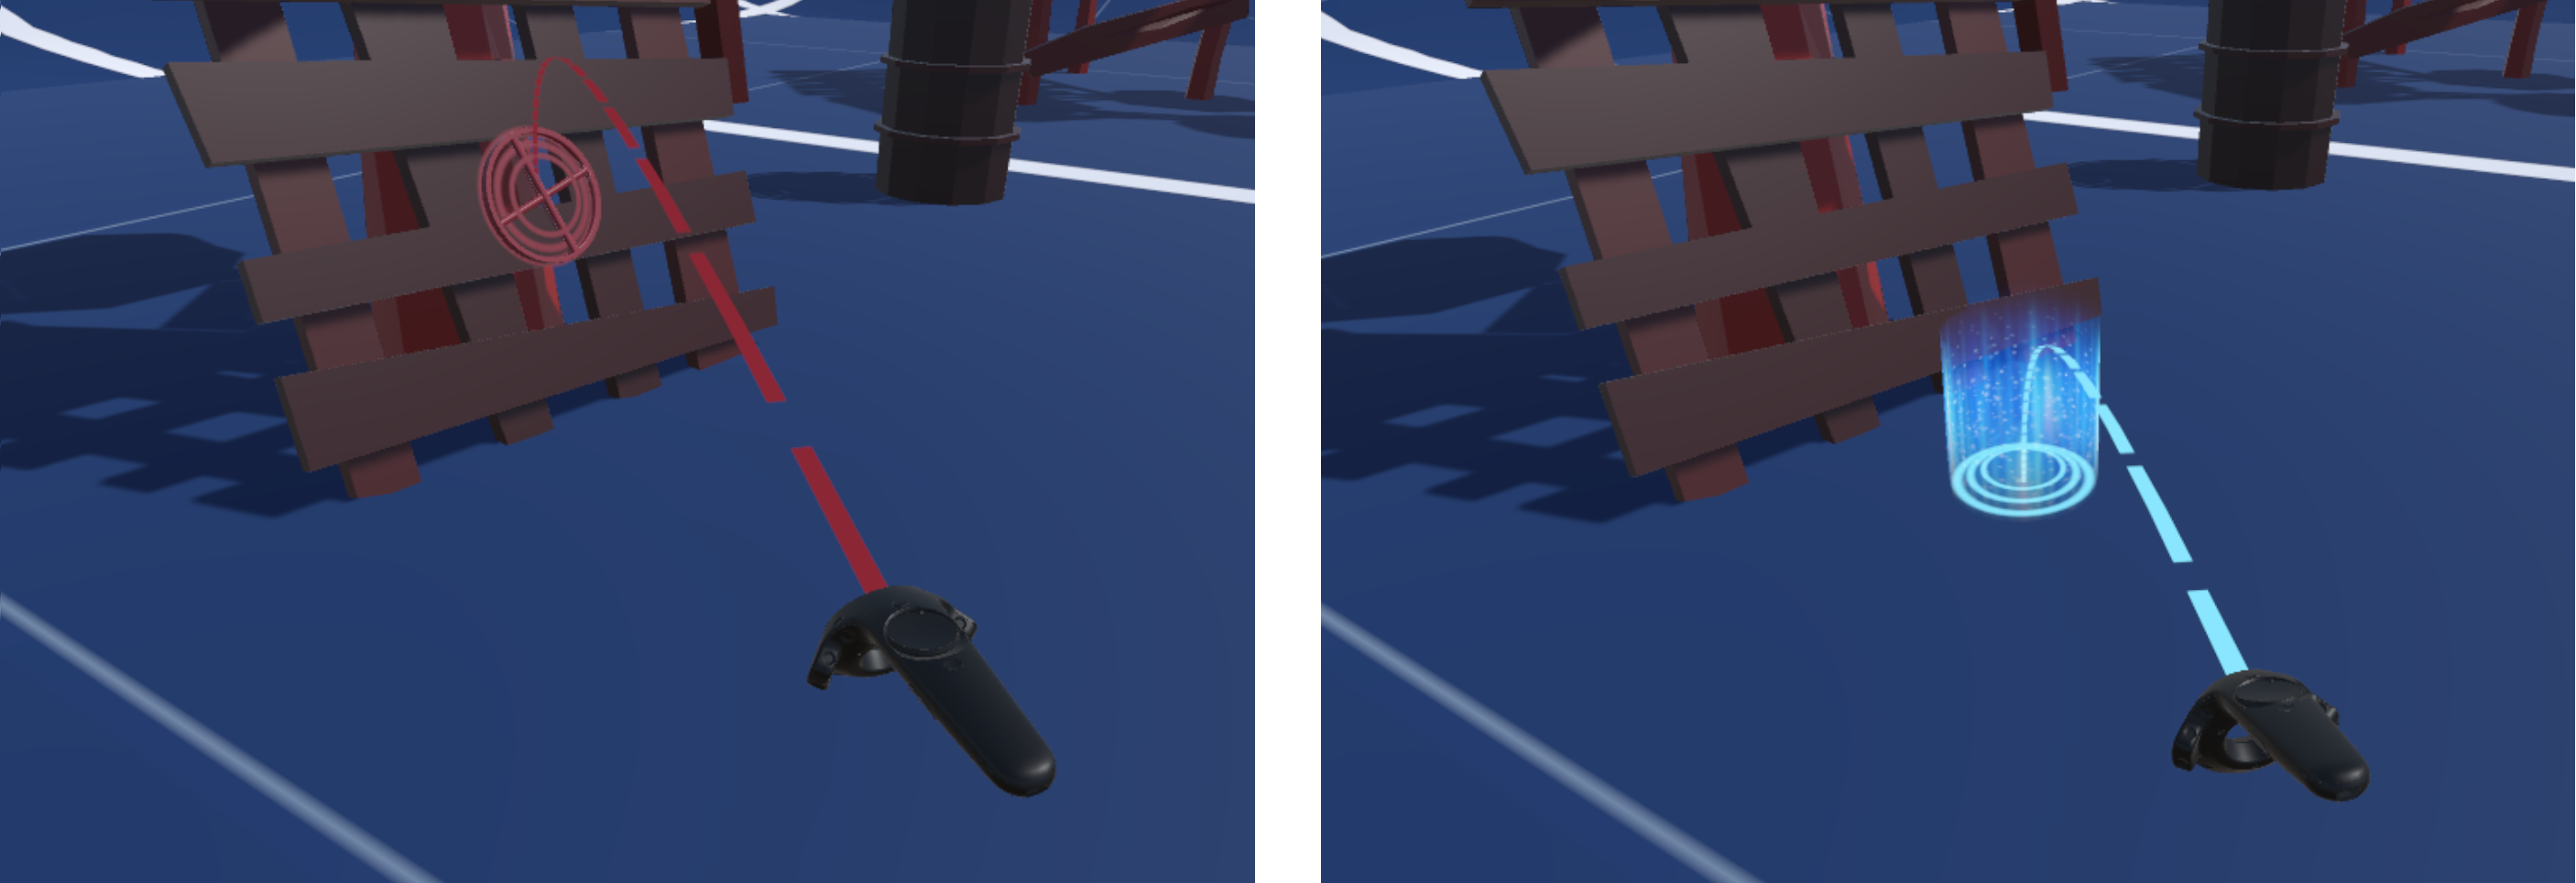
\includegraphics[width=1\textwidth]{img/implemented_teleportation.png}
\caption{The color of teleportation curve was changed from blue to red when the teleportation path was interrupted by one of the objects.}
\label{fig:tpimplementation}
\end{figure}

The goal for the user was to teleport closely to one of the objects in the virtual environment. Next, he had to lean his head towards the object with the purpose of colliding with it. Once the collision was detected, one of the implemented solutions to the problem of VR head collisions was activated. Finally, when the user left the object's boundaries due to the workings of the method, the object's color was changed to green. The green color indicated that the interaction with this object was completed successfully. The user had to repeat the process with each one of the 10 objects until every obstacle was turned green. Because of the need to test four different solutions to the problem of VR head collisions, four different  virtual environments were prepared for the study. All virtual environments were visually identical to each other, with the same placement of the 10 virtual obstacles. The only difference between them was the method of handling VR head collisions.

\subsection{Solutions to the problem of VR Head Collisions}

To detect if the collision with the object occurred, a trigger sphere collider \cite{SPHERECOLLIDER} with the radius of 0.1 m was attached to the user's virtual head. For handling head collisions, four different solutions were implemented: screen fade, delayed push-back, instant push-back, and teleportation. The solutions were implemented by replicating the mechanisms seen in popular VR applications. In the screen fade method, the whole screen gradually faded to black in the span of a second when the collision was detected. Once the user left the object's boundaries by retracting his head back, the object's color was changed from red to green, and the screen gradually returned back to normal in the span of a second (see Figure \ref{fig:fadeimplementation}). 

\begin{figure}[th]
\centering
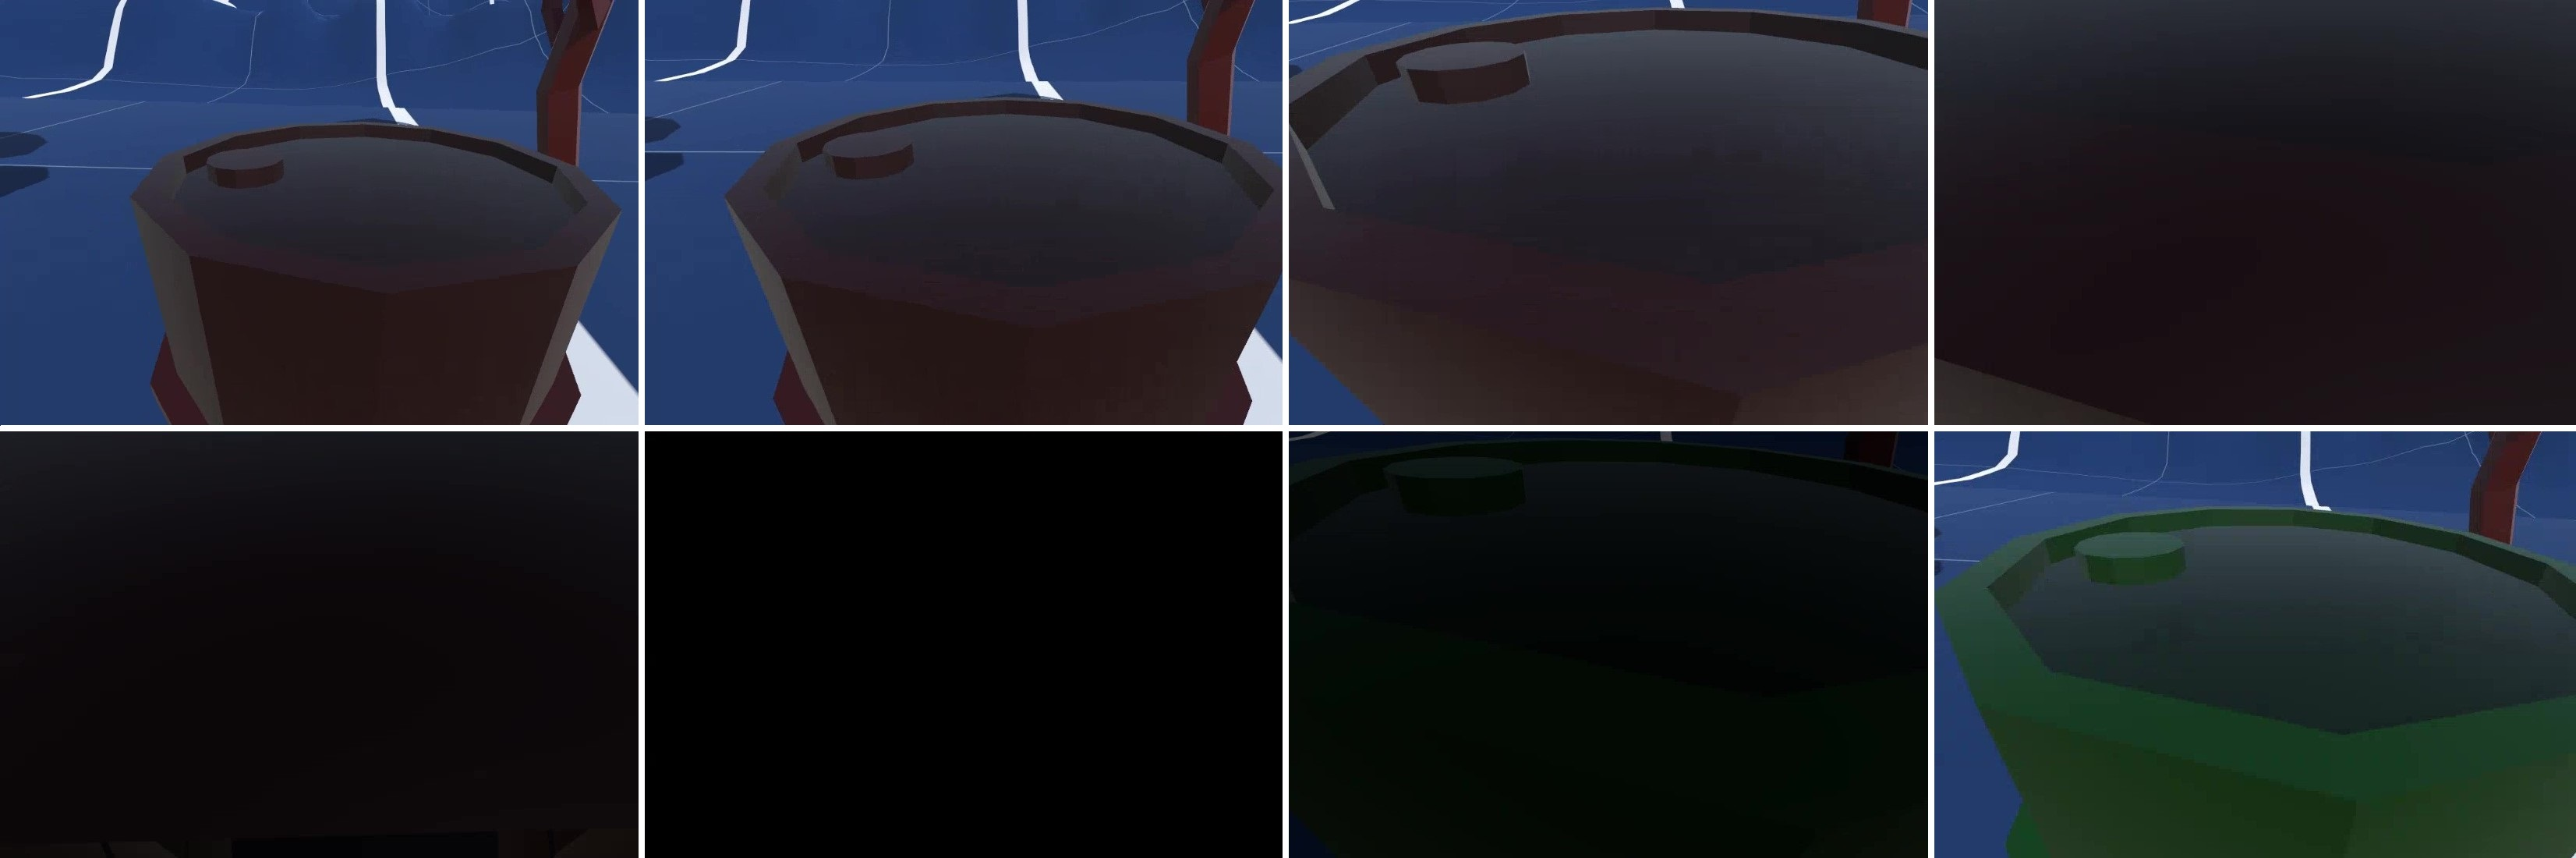
\includegraphics[width=1\textwidth]{img/fade_implementation.jpg}
\caption{A time slice of the implemented screen fade method. The images are ordered from left-to-right and top-to-bottom.}
\label{fig:fadeimplementation}
\end{figure}

The implementation of the delayed push-back method was more complicated and required more steps. In every frame of the application, the collision-free headset position was saved to a variable if the user was not colliding with any object at the moment. After the collision was detected and maintained for the duration of a second, a collision vector between the last collision-free headset position and the current headset position was calculated. The user's position was then pushed back in the direction of the normalized collision vector with the speed of 1 m/s. The push-back effect was working until the user left the object's boundaries. During the duration of the effect, the head tracking system was fully functional and the user could still move his head in every direction. The color was changed to green once the user left the object's boundaries (see Figure \ref{fig:delayedimplementation}).

\begin{figure}[th]
\centering
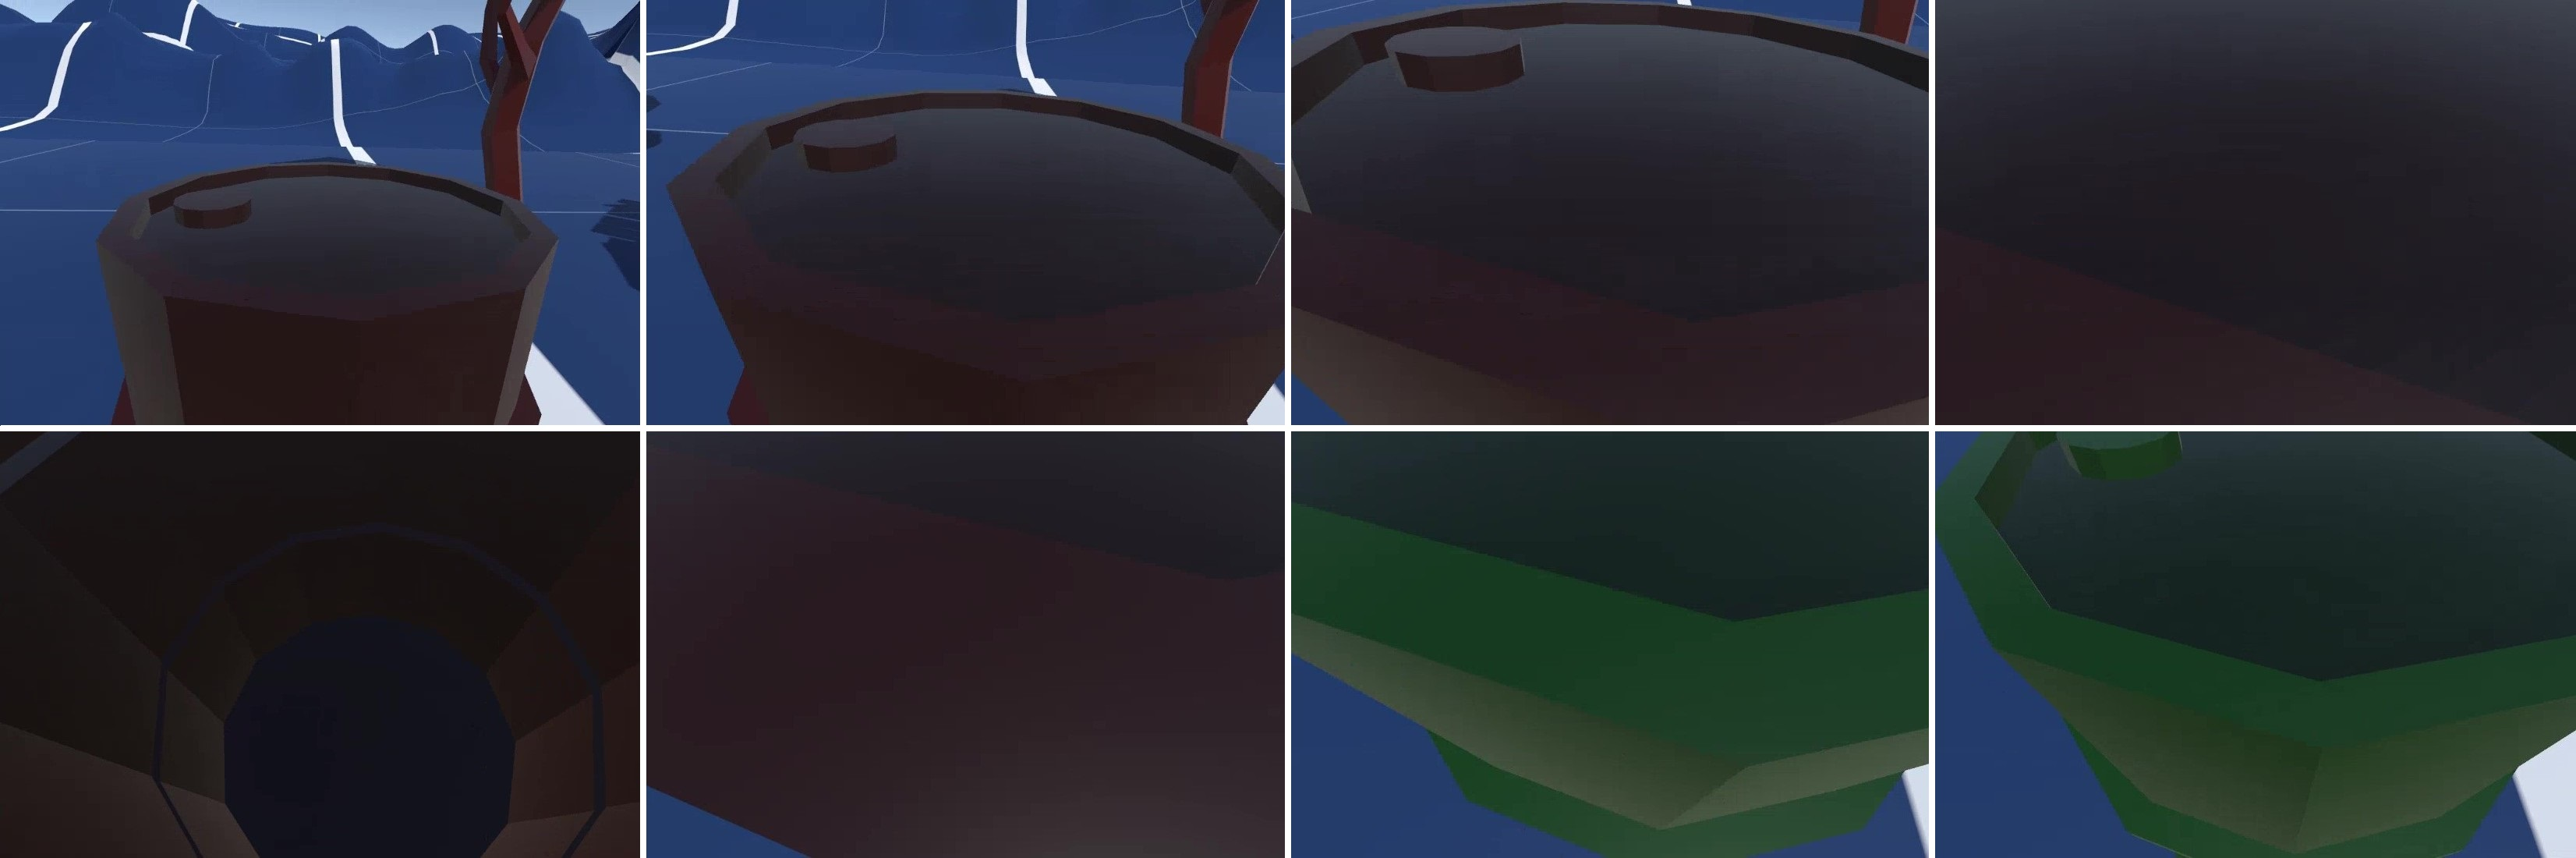
\includegraphics[width=1\textwidth]{img/delayed_implementation.jpg}
\caption{A time slice of the implemented delayed push-back method. The images are ordered from left-to-right and top-to-bottom.}
\label{fig:delayedimplementation}
\end{figure}

The implementation of the instant push-back method was similar to the delayed push-back with a couple of small differences. The collision vector was not normalized, and there was no delay before moving the player's position. In every frame of application, the user was instantly pushed back to the last collision-free position if the collision was detected. To change the color of the object to green, the user had to keep pushing his head in the direction of the collision for the duration of a second (see Figure \ref{fig:instantimplementation}). 

\begin{figure}[th]
\centering
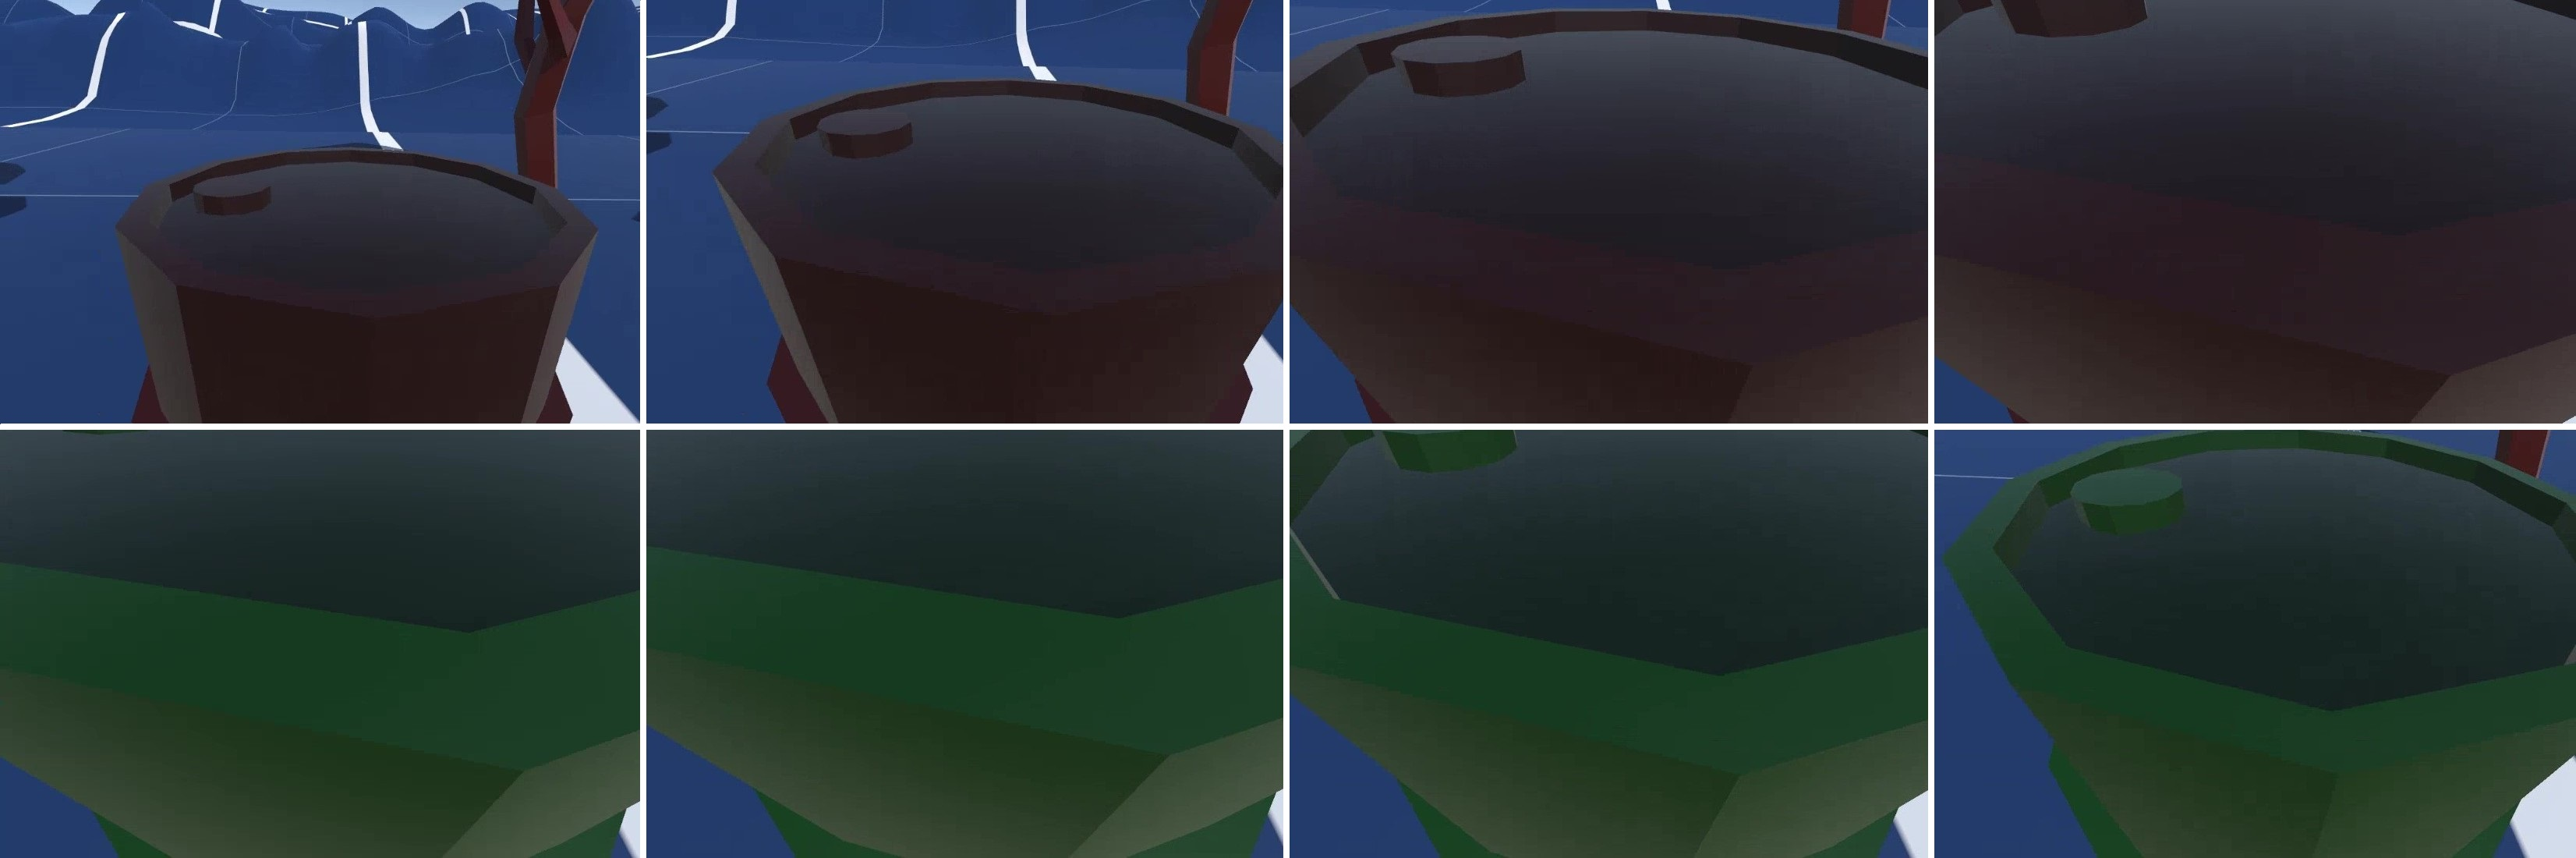
\includegraphics[width=1\textwidth]{img/instant_implementation.jpg}
\caption{A time slice of the implemented instant push-back method. The images are ordered from left-to-right and top-to-bottom.}
\label{fig:instantimplementation}
\end{figure}

In the teleportation technique, the collision vector was also not normalized, and this time there was a delay before the method started working. After the collision was detected and maintained for the duration of a second, the screen blinked for a moment to black, and the user was instantly teleported to the last collision-free position. Once the teleportation occurred, the object's color was changed from red to green (see Figure \ref{fig:teleportimplementation}).

\begin{figure}[th]
\centering
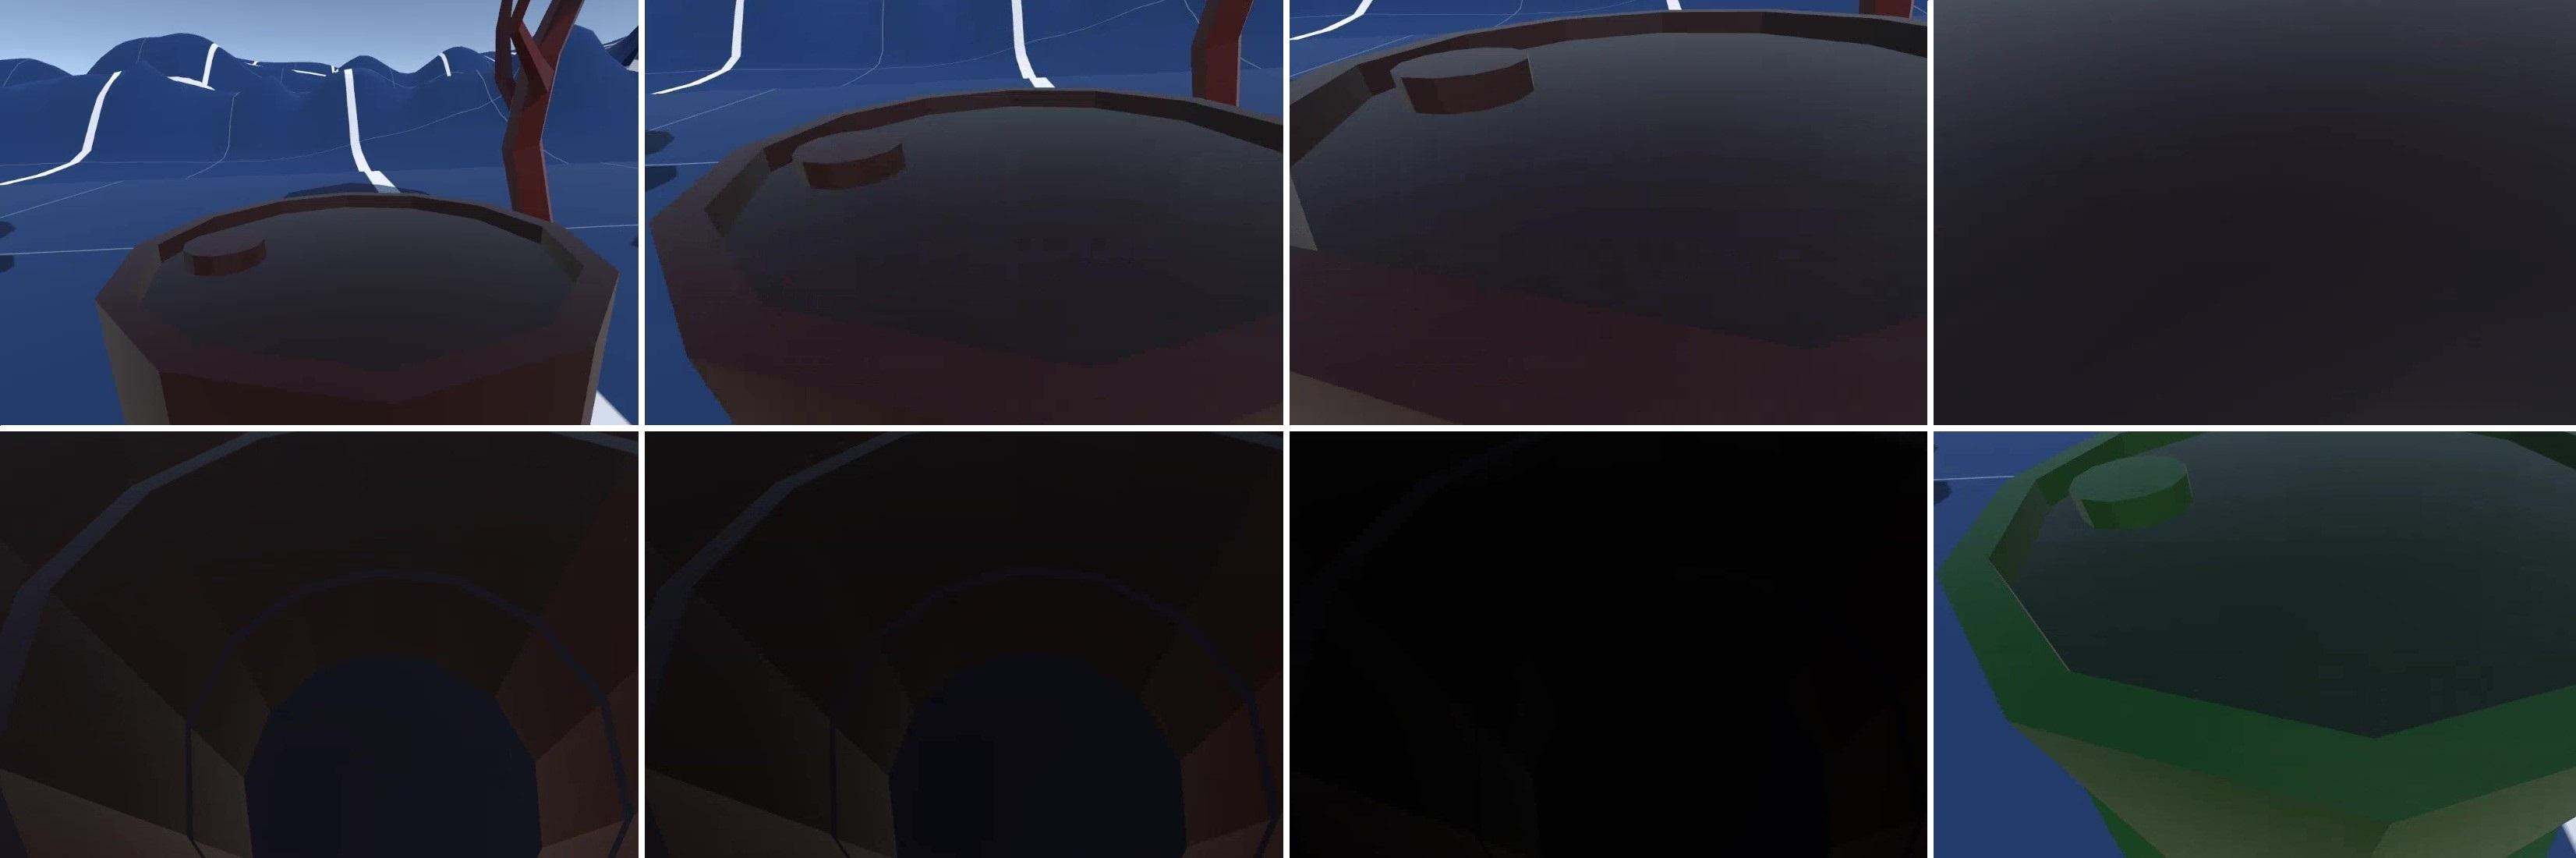
\includegraphics[width=1\textwidth]{img/teleport_implementation.jpg}
\caption{A time slice of the implemented teleportation method. The images are ordered from left-to-right and top-to-bottom.}
\label{fig:teleportimplementation}
\end{figure}

\section{Experiment}

The study employed a within-subject design. The independent variable was the solution to the VR head collisions problem, and it had four levels: screen fade, object fade, camera collider, camera push-back. Due to time constraints, the participants were required to complete the whole experiment with every method in one sitting. For each participant, the order of tested solutions was assigned randomly with Latin Square counterbalancing, where each combination could only be used once.

\subsection{Equipment}

The experiment took place in teaching laboratories with play spaces of approximately 3m x 3m. The participants were equipped with the HTC Vive head-mounted display and its 6DoF hand controller. HTC Vive provides a refresh rate of 90 Hz and a resolution of 2160 x 1200 pixels (1080 x 1200 pixels per eye) with 110$\textsuperscript{o}$ diagonal field of view. Additionally, two Base Stations of the HTC Vive Lighthouse System were used for tracking the head's position and rotation in a 3D environment, which was an integral part of the experiment. A laptop equipped with Nvidia GeForce GTX 1050ti graphic card, 8GB of main memory, and 3.5 GHz Intel Core i5 processor was used for running the implemented VR application. During the experiment, the VR application run at stable 90 frames per second.

\subsection{Participants}

20 participants (3 females, 17 males) aged between 13 and 26 (\textit{M} = 19.65, \textit{SD} = 5.29) were recruited for the study. 12 of them were students of Computer Science master's degree (3 females, 9 males) aged between 23 and 26 (\textit{M} = 23.92, \textit{SD} = 1.08). The rest consisted of children from primary schools (8 males) aged between 13 and 14 (\textit{M} = 13.25, \textit{SD} = 0.46). 9 participants reported that they never experienced motion sickness. This group was particularly instructed about the symptoms of VR sickness. 40\% of the participants have never used a VR headset before and were instructed in details how to use one. See Figure \ref{fig:demographic_charts} for additional charts illustrating the background of the participants.

\begin{figure}[th]
\centering
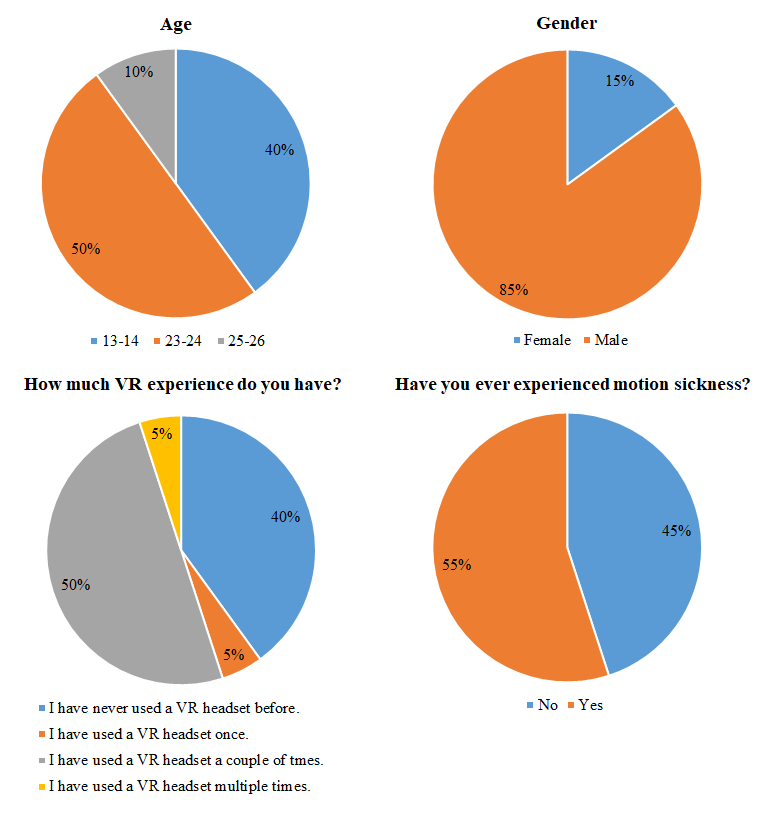
\includegraphics[width=0.99\textwidth]{img/demographic_charts.png}
\caption{A couple of pie charts illustrating the background of the participants.}
\label{fig:demographic_charts}
\end{figure}

\subsection{Procedure}

Upon arriving in the teaching laboratory where the experiment took place, the participants were given a broad overview of the research problem. They were introduced to the main goal of the study and instructed about the task they had to do while present in the virtual environment. Because only a single HTC Vive equipment was available, the participants had to take turns to complete the experiment. Before equipping the headset, the participants were asked to fill in a demographic questionnaire (see Appendix A) about age, gender, previous experiences with motion sickness, and previous experiences with VR headsets.

Once a participant finished filling in the demographic questionnaire and was acquainted with the instructions, he equipped the headset and started testing one of the solutions to the problem of VR head collisions (see Figure \ref{fig:equipment}). His assigned task was to collide with every obstacle in the presented virtual environment. The participant was not told which solution he is testing, and he had to discover on his own how the method is working. Once he successfully collided with the object and observed the effects of the method, the obstacle's color was changed from red to green. 

The participant tested the method until every obstacle in the virtual environment was turned green. On average, it took the participants 2.37 (\textit{SD} = 0.62) minutes to complete this task. Once done, the participant was asked to take off the headset and fill in a post-test questionnaire (see Appendix B). In this questionnaire he described what VR sickness symptoms he felt during the experiment, answered to six questions about the sense of presence, and rated the tested method with eight usability factors. Once the post-test questionnaire was finished, the participant moved on to test the next method. He repeated this process until each of the four methods were tested in this manner. Every participant tested the methods in a unique order.

\begin{figure}[th]
\centering
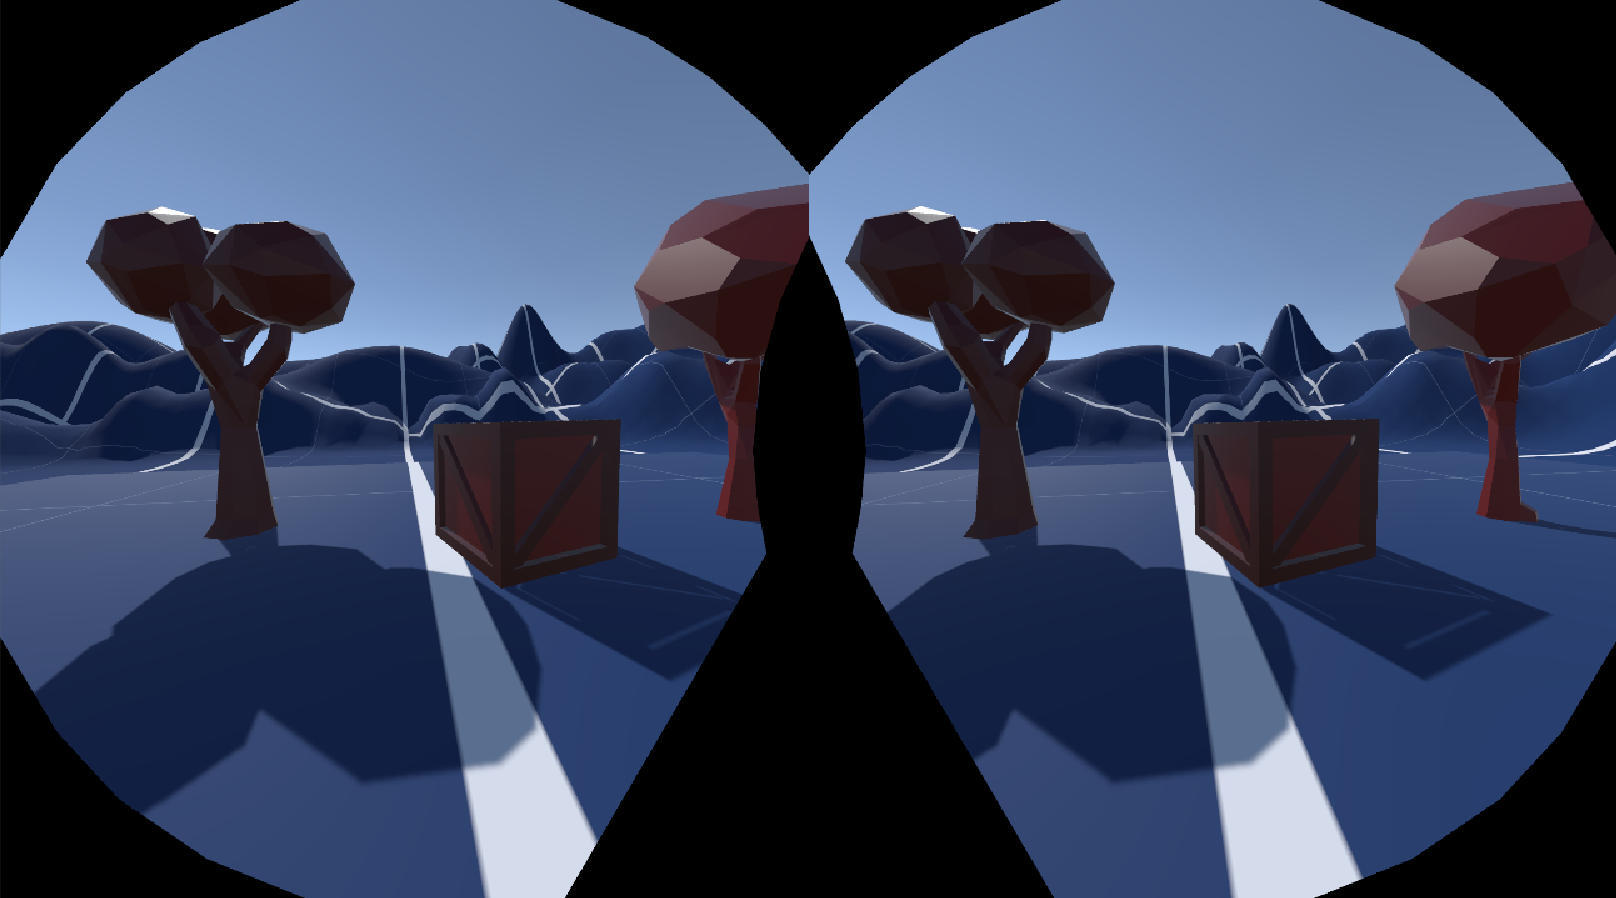
\includegraphics[width=1\textwidth]{img/equipment.png}
\caption{The participants were equipped with the HTC Vive headset and its 6DoF hand controller.}
\label{fig:equipment}
\end{figure}